\section{Dynamic Heap Memory Management}
Always rely on library classes for managing resource handling.

\subsection{When ist Heap Memory used?}
\begin{itemize}
  \itemsep -0.5em 
  \item Stack memory is scarce, most of the time about 1-2MB
  \item It might be needed for creating object structures.
  \item Also needed for polymorphic factory functions to class hierarchies.
  \item Resource Acquisition Initialization (RAII) Idiom
\end{itemize}

\subsection{Legacy Heap Memory}
\textbf{Dont use this!}\\
C++ allows allocating objects on the heap directly. If done manually, you are responsible for deallocation and risk undefined behaviour. This will mostly result in Memory leaks, Dangling pointers and Double deletes. The programmer is responsible to allocate and free all the memory used.
\begin{lstlisting}[language=C++]
// dont use new / delete
auto pr = new int{};
std::cout << *ptr << '\n';
delete ptr;
\end{lstlisting}

\subsection{Modern Heap Management (C++11)}
In the modern C++ world we can use smart pointers, which are C++ templates, to make memory management easier. With these smart pointers we dont have to call "delete ptr;" by ourselfs. Still: always prefer storing the value locally as value-type variable (Stack-based or member).
\begin{itemize}
  \itemsep -0.5em 
  \item Delete Pointer - must never be called.
  \item Unique Pointer - for unshared Heap Memory (cant be copied, can be moved).
  \item Shared Pointer - for shared Heap Memory (work as Java references, can be copied and moved).
  \item If the last "shared\_ptr" handle gets destroyed, the allocated object gets deleted.
  \item Shared Pointer have the problem of cycles. For this reason there is a "weak\_ptr" to break the cycles.
\end{itemize}


\subsubsection{std::unique\_ptr<T>}
\begin{itemize}
  \itemsep -0.5em 
  \item defined in \lstinline|#include <memory>|
  \item Uses the factory method \lstinline|std::make_unique<T>()|
  \item Used for unshared heap memory
  	\SubItem{Or for local stuff that must be on the heap}
  	\SubItem{Can be returned from a factory function}
  \item Only a single owner exists
  \item Not the best for class hierarchies
  \item Can not be copied
\end{itemize}

\textbf{Use Cases}
\begin{itemize}
  \itemsep -0.5em 
  \item As member variable
  \item As local variable
\end{itemize}

\begin{lstlisting}
#include <iostream>
#include <memory>
#include <utility>

std::unique_ptr<int> create(int i) { // transfer of ownership through return by value
  return std::make_unique<int>(i); 
}

int main() {
  std::cout << std::boolalpha;
  auto pi = create(42);
  std::cout << "*pi = " << *pi << '\n';
  std::cout << "pi.valid? " << static_cast<bool>(pi) << '\n';
  auto pj = std::move(pi); // explicit transfer of ownership
  std::cout << "*pj = " << *pj << '\n';
  std::cout << "pi.valid? " << static_cast<bool>(pi) << '\n';
}
\end{lstlisting}


\subsubsection{shared\_ptr<T>}
\begin{itemize}
	\itemsep -0.5em
	\item Works more like a Java reference and allows multiple owners.
	\item Therefore it can be copied, passed around.
	\item Has a reference counter on the heap object. Object gets destructed as soon as there are no references left.
	\item The pointer is \lstinline|std::shared_ptr| and associates objects of Type T using \lstinline|std::make_shared<T>()|.
	\item If instances of a class hierarchy are always represented by a \lstinline|std::shared_ptr<base>| but created through \lstinline|std::make_shared<concrete>()| the destructor no longer needs to be virtual.
	\item Can lead to object cycles no longer cleared, because of circular dependency
\end{itemize}


\begin{lstlisting}[language=C++]
struct Article { 
	Article(std::string title, std::string content);
 	//..
};
Article cppExam{"How to pass CPl?", "In order to pass the C++ exam, you have to..."};
std::shared_ptr<Article> abcPtr = std::make_shared<Article>("Alphabet", "ABCDEFXYZ");
\end{lstlisting}

\textbf{Use Cases}
\begin{itemize}
  \itemsep 0em 
  \item If you really need heap-allocated objects, because you create your own object networks
  \item  If you need to support run-time polymorphic container contents or class members that can not be passed as reference, e.g., because of lifetime issues 
  \item Factory functions returning std::shared\_ptr for heap allocated objects.
  \item  But first check if alternatives are viable:
	\SubItem{(const) references as parameter types or class members}
	\SubItem{Plain member objects or containers with plain class instances}
\end{itemize}

The usage is counted on the referenced object to keep track of how many reference currently point to this object on the heap.

\begin{figure}[h!]
  \center
  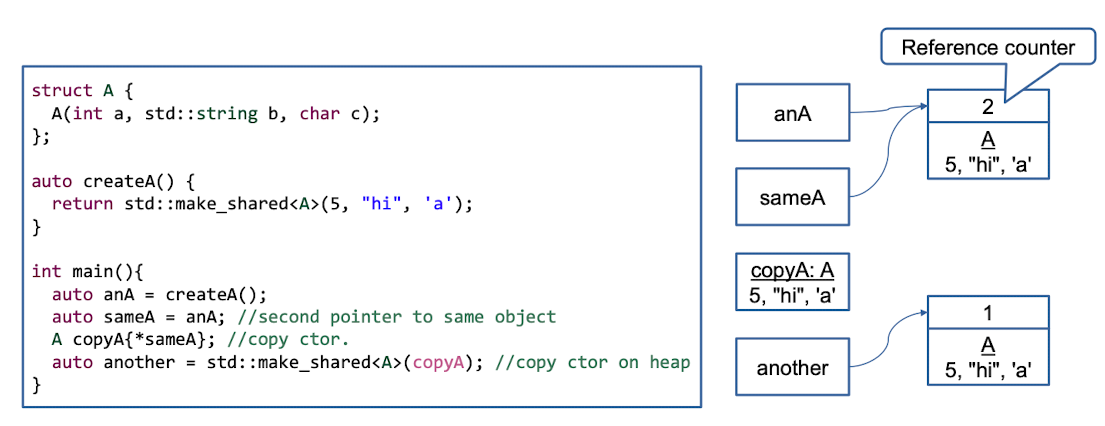
\includegraphics[width=0.8\linewidth]{sharedptr}
  \caption{Shared Pointer}
\end{figure}


\subsubsection{std::weak\_ptr<T>}
\begin{itemize}
  \itemsep -0.5em 
  \item The \lstinline|shared_ptr<T>| cycles need to be broken for nesting and object networks and this can be done with \lstinline|weak_ptr<T>|.
  \item \lstinline|weak_ptr| does not allow direct access to the object
  \item A \lstinline|weak_ptr| does not know weather the pointer is still alive
  \item with \lstinline|lock()| to the object can be acquired if alive. 
\end{itemize}

\begin{figure}[h!]
  \centering
  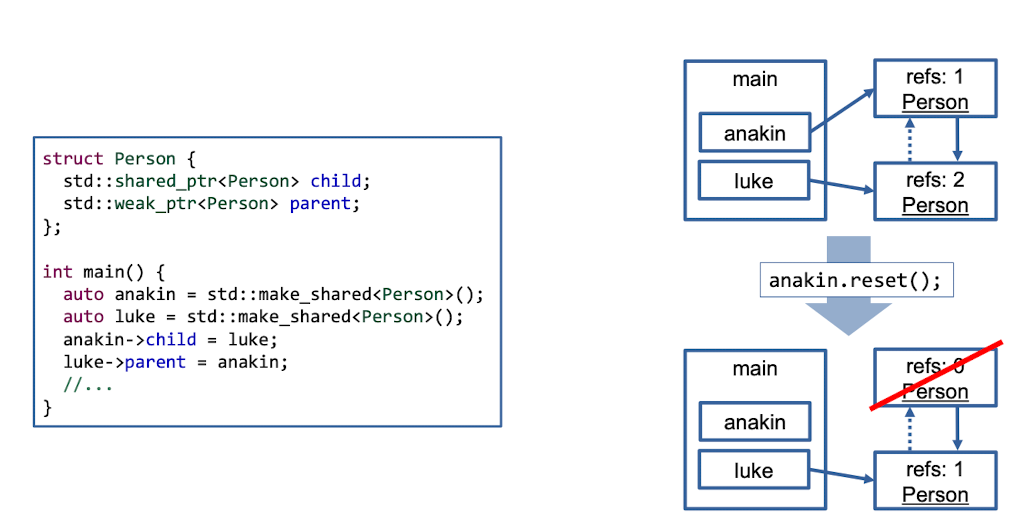
\includegraphics[width=0.75\linewidth]{weakptr}
  \caption{Weak Pointer}
\end{figure}

\textbf{Access with std::weak\_ptr}\\
As mentioned a weak ptr does not know whether the pointee is still alive. \lstinline|std::weak_ptr::lock()| return a \lstinline|std::shared_ptr| that either points to the alive pointee or is empty.

\begin{figure}[h!]
  \center
  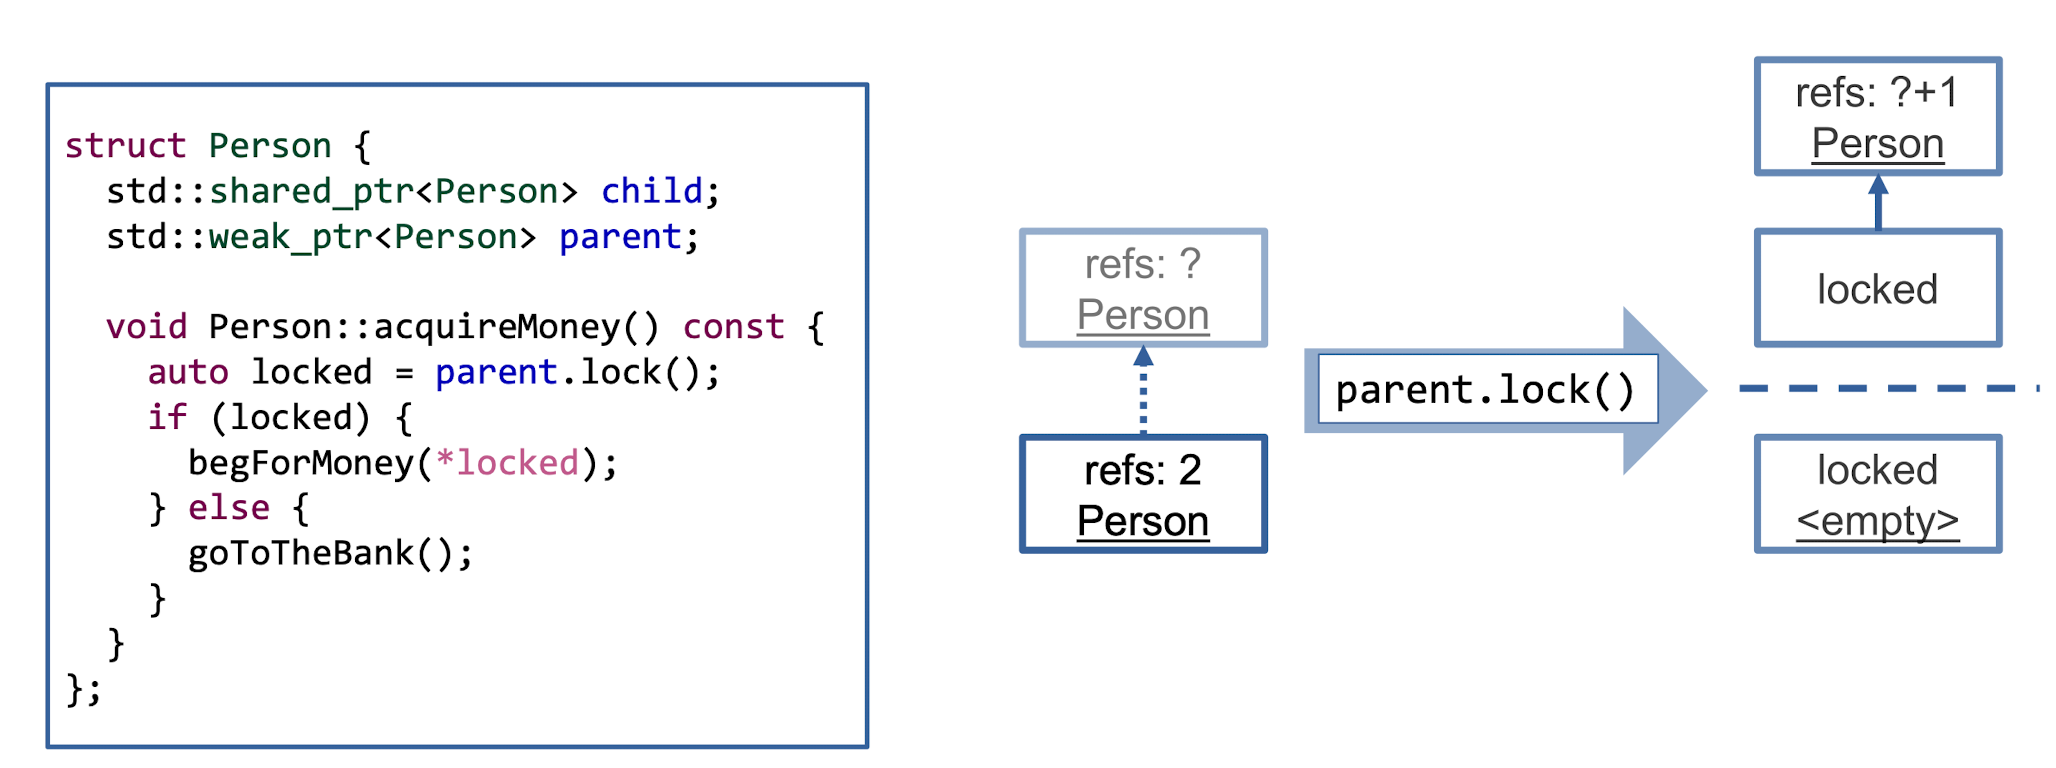
\includegraphics[width=0.75\linewidth]{weakptraccess}
  \caption{Shared Pointer Access Check with Lock}
\end{figure}

\textbf{Spawning Children from parents}\\
This can be done if we inherit from \lstinline|std::enable_shared_from_this<T>|. Then we can access the function \lstinline|weak_from_this();| to create a reference to the parent.

\begin{figure}[h!]
  \center
  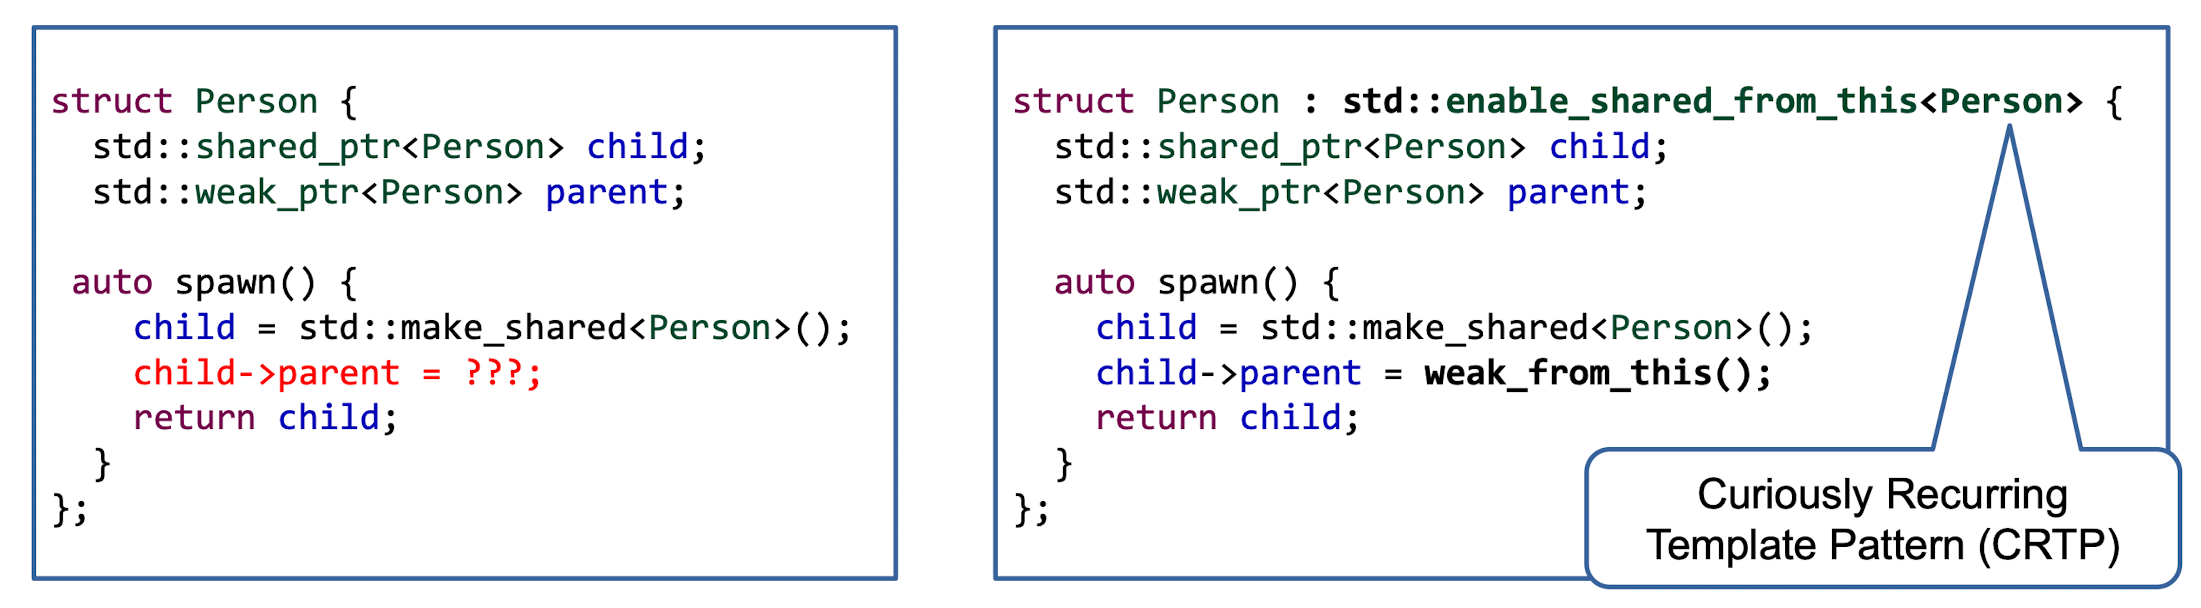
\includegraphics[width=0.75\linewidth]{enableshared}
  \caption{Enable Shared Parent Creation}
\end{figure}

